% Options for packages loaded elsewhere
\PassOptionsToPackage{unicode}{hyperref}
\PassOptionsToPackage{hyphens}{url}
%
\documentclass[
]{article}
\usepackage{amsmath,amssymb}
\usepackage{iftex}
\ifPDFTeX
  \usepackage[T1]{fontenc}
  \usepackage[utf8]{inputenc}
  \usepackage{textcomp} % provide euro and other symbols
\else % if luatex or xetex
  \usepackage{unicode-math} % this also loads fontspec
  \defaultfontfeatures{Scale=MatchLowercase}
  \defaultfontfeatures[\rmfamily]{Ligatures=TeX,Scale=1}
\fi
\usepackage{lmodern}
\ifPDFTeX\else
  % xetex/luatex font selection
\fi
% Use upquote if available, for straight quotes in verbatim environments
\IfFileExists{upquote.sty}{\usepackage{upquote}}{}
\IfFileExists{microtype.sty}{% use microtype if available
  \usepackage[]{microtype}
  \UseMicrotypeSet[protrusion]{basicmath} % disable protrusion for tt fonts
}{}
\makeatletter
\@ifundefined{KOMAClassName}{% if non-KOMA class
  \IfFileExists{parskip.sty}{%
    \usepackage{parskip}
  }{% else
    \setlength{\parindent}{0pt}
    \setlength{\parskip}{6pt plus 2pt minus 1pt}}
}{% if KOMA class
  \KOMAoptions{parskip=half}}
\makeatother
\usepackage{xcolor}
\usepackage[margin=1in]{geometry}
\usepackage{color}
\usepackage{fancyvrb}
\newcommand{\VerbBar}{|}
\newcommand{\VERB}{\Verb[commandchars=\\\{\}]}
\DefineVerbatimEnvironment{Highlighting}{Verbatim}{commandchars=\\\{\}}
% Add ',fontsize=\small' for more characters per line
\usepackage{framed}
\definecolor{shadecolor}{RGB}{248,248,248}
\newenvironment{Shaded}{\begin{snugshade}}{\end{snugshade}}
\newcommand{\AlertTok}[1]{\textcolor[rgb]{0.94,0.16,0.16}{#1}}
\newcommand{\AnnotationTok}[1]{\textcolor[rgb]{0.56,0.35,0.01}{\textbf{\textit{#1}}}}
\newcommand{\AttributeTok}[1]{\textcolor[rgb]{0.13,0.29,0.53}{#1}}
\newcommand{\BaseNTok}[1]{\textcolor[rgb]{0.00,0.00,0.81}{#1}}
\newcommand{\BuiltInTok}[1]{#1}
\newcommand{\CharTok}[1]{\textcolor[rgb]{0.31,0.60,0.02}{#1}}
\newcommand{\CommentTok}[1]{\textcolor[rgb]{0.56,0.35,0.01}{\textit{#1}}}
\newcommand{\CommentVarTok}[1]{\textcolor[rgb]{0.56,0.35,0.01}{\textbf{\textit{#1}}}}
\newcommand{\ConstantTok}[1]{\textcolor[rgb]{0.56,0.35,0.01}{#1}}
\newcommand{\ControlFlowTok}[1]{\textcolor[rgb]{0.13,0.29,0.53}{\textbf{#1}}}
\newcommand{\DataTypeTok}[1]{\textcolor[rgb]{0.13,0.29,0.53}{#1}}
\newcommand{\DecValTok}[1]{\textcolor[rgb]{0.00,0.00,0.81}{#1}}
\newcommand{\DocumentationTok}[1]{\textcolor[rgb]{0.56,0.35,0.01}{\textbf{\textit{#1}}}}
\newcommand{\ErrorTok}[1]{\textcolor[rgb]{0.64,0.00,0.00}{\textbf{#1}}}
\newcommand{\ExtensionTok}[1]{#1}
\newcommand{\FloatTok}[1]{\textcolor[rgb]{0.00,0.00,0.81}{#1}}
\newcommand{\FunctionTok}[1]{\textcolor[rgb]{0.13,0.29,0.53}{\textbf{#1}}}
\newcommand{\ImportTok}[1]{#1}
\newcommand{\InformationTok}[1]{\textcolor[rgb]{0.56,0.35,0.01}{\textbf{\textit{#1}}}}
\newcommand{\KeywordTok}[1]{\textcolor[rgb]{0.13,0.29,0.53}{\textbf{#1}}}
\newcommand{\NormalTok}[1]{#1}
\newcommand{\OperatorTok}[1]{\textcolor[rgb]{0.81,0.36,0.00}{\textbf{#1}}}
\newcommand{\OtherTok}[1]{\textcolor[rgb]{0.56,0.35,0.01}{#1}}
\newcommand{\PreprocessorTok}[1]{\textcolor[rgb]{0.56,0.35,0.01}{\textit{#1}}}
\newcommand{\RegionMarkerTok}[1]{#1}
\newcommand{\SpecialCharTok}[1]{\textcolor[rgb]{0.81,0.36,0.00}{\textbf{#1}}}
\newcommand{\SpecialStringTok}[1]{\textcolor[rgb]{0.31,0.60,0.02}{#1}}
\newcommand{\StringTok}[1]{\textcolor[rgb]{0.31,0.60,0.02}{#1}}
\newcommand{\VariableTok}[1]{\textcolor[rgb]{0.00,0.00,0.00}{#1}}
\newcommand{\VerbatimStringTok}[1]{\textcolor[rgb]{0.31,0.60,0.02}{#1}}
\newcommand{\WarningTok}[1]{\textcolor[rgb]{0.56,0.35,0.01}{\textbf{\textit{#1}}}}
\usepackage{graphicx}
\makeatletter
\def\maxwidth{\ifdim\Gin@nat@width>\linewidth\linewidth\else\Gin@nat@width\fi}
\def\maxheight{\ifdim\Gin@nat@height>\textheight\textheight\else\Gin@nat@height\fi}
\makeatother
% Scale images if necessary, so that they will not overflow the page
% margins by default, and it is still possible to overwrite the defaults
% using explicit options in \includegraphics[width, height, ...]{}
\setkeys{Gin}{width=\maxwidth,height=\maxheight,keepaspectratio}
% Set default figure placement to htbp
\makeatletter
\def\fps@figure{htbp}
\makeatother
\setlength{\emergencystretch}{3em} % prevent overfull lines
\providecommand{\tightlist}{%
  \setlength{\itemsep}{0pt}\setlength{\parskip}{0pt}}
\setcounter{secnumdepth}{-\maxdimen} % remove section numbering
\ifLuaTeX
  \usepackage{selnolig}  % disable illegal ligatures
\fi
\IfFileExists{bookmark.sty}{\usepackage{bookmark}}{\usepackage{hyperref}}
\IfFileExists{xurl.sty}{\usepackage{xurl}}{} % add URL line breaks if available
\urlstyle{same}
\hypersetup{
  pdftitle={Statistical Computing},
  pdfauthor={Tinotenda Mutsemi (MTSTIN007)},
  hidelinks,
  pdfcreator={LaTeX via pandoc}}

\title{Statistical Computing}
\usepackage{etoolbox}
\makeatletter
\providecommand{\subtitle}[1]{% add subtitle to \maketitle
  \apptocmd{\@title}{\par {\large #1 \par}}{}{}
}
\makeatother
\subtitle{Assignment 2}
\author{Tinotenda Mutsemi (MTSTIN007)}
\date{2024-03-12}

\begin{document}
\maketitle

\hypertarget{question-1}{%
\section{Question 1}\label{question-1}}

The true integral value is given by:

\[ \int_0^1x^3dx = [x^4/4]_0^1 = 0.25 \]

\hypertarget{question-1a}{%
\subsection{Question 1a}\label{question-1a}}

Now we approximate the integral using uniform distribution. We define
fx, sample 1000 uniform values between 0 and 1, and calculate the mean
value of the function. The integral estimate is the area of the
rectangle, mean value multiplied by the interval difference. We get an
estimate of 0.246, with a standard error of 0.008893

\begin{Shaded}
\begin{Highlighting}[]
\CommentTok{\#fx function def}
\NormalTok{fx }\OtherTok{\textless{}{-}} \ControlFlowTok{function}\NormalTok{(x, n)\{}
  \FunctionTok{return}\NormalTok{(x}\SpecialCharTok{**}\NormalTok{n)}
\NormalTok{\}}


\NormalTok{N }\OtherTok{\textless{}{-}} \DecValTok{1000}
\NormalTok{a }\OtherTok{\textless{}{-}} \DecValTok{0}
\NormalTok{b }\OtherTok{\textless{}{-}} \DecValTok{1}
\end{Highlighting}
\end{Shaded}

\begin{Shaded}
\begin{Highlighting}[]
\CommentTok{\#sample 1000 uniform values between 0 and 1}
\FunctionTok{set.seed}\NormalTok{(}\DecValTok{123}\NormalTok{)}
\NormalTok{x\_sample\_unif }\OtherTok{\textless{}{-}} \FunctionTok{runif}\NormalTok{(N, }\DecValTok{0}\NormalTok{, }\DecValTok{1}\NormalTok{)}

\NormalTok{y\_sample }\OtherTok{\textless{}{-}} \FunctionTok{fx}\NormalTok{(}\AttributeTok{x =}\NormalTok{ x\_sample\_unif, }\AttributeTok{n =} \DecValTok{3}\NormalTok{)}

\NormalTok{mean\_sample }\OtherTok{\textless{}{-}} \FunctionTok{sum}\NormalTok{(y\_sample)}\SpecialCharTok{/}\NormalTok{ N}

\NormalTok{intergral\_est }\OtherTok{\textless{}{-}}\NormalTok{ mean\_sample }\SpecialCharTok{*}\NormalTok{ (b }\SpecialCharTok{{-}}\NormalTok{ a)}
\NormalTok{intergral\_est}
\end{Highlighting}
\end{Shaded}

\begin{verbatim}
## [1] 0.2464137
\end{verbatim}

\begin{Shaded}
\begin{Highlighting}[]
\CommentTok{\#standard error of the estimate}
\FunctionTok{sqrt}\NormalTok{((}\FunctionTok{sum}\NormalTok{((y\_sample }\SpecialCharTok{{-}}\NormalTok{ mean\_sample)}\SpecialCharTok{**}\DecValTok{2}\NormalTok{))}\SpecialCharTok{/}\NormalTok{(N }\SpecialCharTok{*}\NormalTok{ (N}\DecValTok{{-}1}\NormalTok{)))}
\end{Highlighting}
\end{Shaded}

\begin{verbatim}
## [1] 0.008893887
\end{verbatim}

\hypertarget{question-1b}{%
\subsection{Question 1b}\label{question-1b}}

For accept reject sampling, we use a power law distribution as a
proposal distribution. We sample 1000 values from the proposal
distribution, using the inverse transform sampling method. We then
calculate the acceptance probability (ratio of target to proposal). We
then sample from a uniform distribution and accept the sampled values
that are less than the acceptance probability. The estimate of the
integral is the mean of the accepted values. We get an estimate of
0.115, with a standard error of 0.000199

\begin{Shaded}
\begin{Highlighting}[]
\FunctionTok{set.seed}\NormalTok{(}\DecValTok{123}\NormalTok{)}
\CommentTok{\#proposal distribution a power law distribution}
\NormalTok{N }\OtherTok{\textless{}{-}} \DecValTok{10000}

\NormalTok{px }\OtherTok{\textless{}{-}} \ControlFlowTok{function}\NormalTok{(x, k)\{}
  \FunctionTok{return}\NormalTok{((k}\SpecialCharTok{+}\DecValTok{1}\NormalTok{) }\SpecialCharTok{*}\NormalTok{ x}\SpecialCharTok{**}\NormalTok{k)}
\NormalTok{\}}


\NormalTok{px\_inv }\OtherTok{\textless{}{-}} \ControlFlowTok{function}\NormalTok{(y, k)\{}
  \FunctionTok{return}\NormalTok{((y}\SpecialCharTok{/}\NormalTok{(k}\SpecialCharTok{+}\DecValTok{1}\NormalTok{)) }\SpecialCharTok{**}\NormalTok{ (}\DecValTok{1}\SpecialCharTok{/}\NormalTok{k))}
\NormalTok{\}}

\NormalTok{uniform\_sample }\OtherTok{\textless{}{-}} \FunctionTok{runif}\NormalTok{(N, }\DecValTok{0}\NormalTok{, }\DecValTok{1}\NormalTok{)}

\CommentTok{\#inverse transform sampling}
\NormalTok{x\_sample\_ar }\OtherTok{\textless{}{-}} \FunctionTok{px\_inv}\NormalTok{(uniform\_sample, }\AttributeTok{k =} \FloatTok{2.5}\NormalTok{)}

\CommentTok{\#prob of acceptance}
\NormalTok{prob\_accept }\OtherTok{\textless{}{-}} \FunctionTok{fx}\NormalTok{(x\_sample\_ar, }\AttributeTok{n =} \DecValTok{3}\NormalTok{)}\SpecialCharTok{/}\FunctionTok{px}\NormalTok{(x\_sample\_ar, }\AttributeTok{k =} \FloatTok{2.5}\NormalTok{)}

\CommentTok{\#sample from uniform distribution}
\NormalTok{u\_sample }\OtherTok{\textless{}{-}} \FunctionTok{runif}\NormalTok{(N, }\DecValTok{0}\NormalTok{, }\DecValTok{1}\NormalTok{)}

\CommentTok{\#acceptance rejection}
\NormalTok{x\_sample\_ar }\OtherTok{\textless{}{-}}\NormalTok{ x\_sample\_ar[u\_sample }\SpecialCharTok{\textless{}}\NormalTok{ prob\_accept]}

\CommentTok{\#take first 1000 values}
\NormalTok{x\_sample\_ar }\OtherTok{\textless{}{-}}\NormalTok{ x\_sample\_ar[}\DecValTok{1}\SpecialCharTok{:}\DecValTok{1000}\NormalTok{]}

\CommentTok{\#find the estimate}
\NormalTok{intergral\_est }\OtherTok{\textless{}{-}} \FunctionTok{sum}\NormalTok{(}\FunctionTok{fx}\NormalTok{(x\_sample\_ar, }\AttributeTok{n =} \DecValTok{3}\NormalTok{))}\SpecialCharTok{/}\FunctionTok{length}\NormalTok{(x\_sample\_ar)}

\NormalTok{intergral\_est}
\end{Highlighting}
\end{Shaded}

\begin{verbatim}
## [1] 0.1152469
\end{verbatim}

\begin{Shaded}
\begin{Highlighting}[]
\CommentTok{\#standard error of the estimate}
\FunctionTok{sqrt}\NormalTok{((}\FunctionTok{sum}\NormalTok{((}\FunctionTok{fx}\NormalTok{(x\_sample\_ar, }\AttributeTok{n =} \DecValTok{3}\NormalTok{) }\SpecialCharTok{{-}}\NormalTok{ intergral\_est)}\SpecialCharTok{**}\DecValTok{2}\NormalTok{))}\SpecialCharTok{/}\NormalTok{(N }\SpecialCharTok{*}\NormalTok{ (N}\DecValTok{{-}1}\NormalTok{)))}
\end{Highlighting}
\end{Shaded}

\begin{verbatim}
## [1] 0.0001993705
\end{verbatim}

\hypertarget{question-1c}{%
\subsection{Question 1c}\label{question-1c}}

For importance sampling, we use the same proposal distribution as in b).
We sample 1000 values from uniform distribution between 0 and 1, use
inverse of the power law distribution to get the values of x. We then
weight the sample values by the ratio of the target and proposal
distribution. We get an estimate of 0.185, with a standard error of
0.000991

\begin{Shaded}
\begin{Highlighting}[]
\CommentTok{\#Importance sampling with the same proposal candidate distribution as px}
\FunctionTok{set.seed}\NormalTok{(}\DecValTok{123}\NormalTok{)}
\NormalTok{N }\OtherTok{\textless{}{-}} \DecValTok{1000}

\CommentTok{\#sample 1000 from px}
\NormalTok{x\_sample\_imp }\OtherTok{\textless{}{-}} \FunctionTok{px\_inv}\NormalTok{(}\FunctionTok{runif}\NormalTok{(N, }\DecValTok{0}\NormalTok{, }\DecValTok{1}\NormalTok{), }\AttributeTok{k =} \FloatTok{2.5}\NormalTok{)}

\CommentTok{\#find the weights}
\NormalTok{weights }\OtherTok{\textless{}{-}} \FunctionTok{fx}\NormalTok{(x\_sample\_imp, }\AttributeTok{n =} \DecValTok{3}\NormalTok{)}\SpecialCharTok{/}\FunctionTok{px}\NormalTok{(x\_sample\_imp, }\AttributeTok{k =} \FloatTok{2.5}\NormalTok{)}

\CommentTok{\#find the estimate}
\NormalTok{intergral\_est }\OtherTok{\textless{}{-}} \FunctionTok{sum}\NormalTok{(weights)}\SpecialCharTok{/}\NormalTok{N}

\NormalTok{intergral\_est}
\end{Highlighting}
\end{Shaded}

\begin{verbatim}
## [1] 0.1851229
\end{verbatim}

\begin{Shaded}
\begin{Highlighting}[]
\CommentTok{\#standard error of the estimate}
\FunctionTok{sqrt}\NormalTok{((}\FunctionTok{sum}\NormalTok{((weights }\SpecialCharTok{{-}}\NormalTok{ intergral\_est)}\SpecialCharTok{**}\DecValTok{2}\NormalTok{))}\SpecialCharTok{/}\NormalTok{(N }\SpecialCharTok{*}\NormalTok{ (N}\DecValTok{{-}1}\NormalTok{)))}
\end{Highlighting}
\end{Shaded}

\begin{verbatim}
## [1] 0.0009912263
\end{verbatim}

\hypertarget{question-1-conclusions}{%
\subsection{Question 1 conclusions}\label{question-1-conclusions}}

The uniform sampling estimate is the closest to the true value of the
integral as it samples from a true uniform (and the target is a CDF)
compared to the inverse of px which is not truly uniform (shown in
figure 1). Importance sampling performs better than just using the
proposal distribution as it places more weight on the values of x that
are closer to the target distribution.

\begin{figure}
\centering
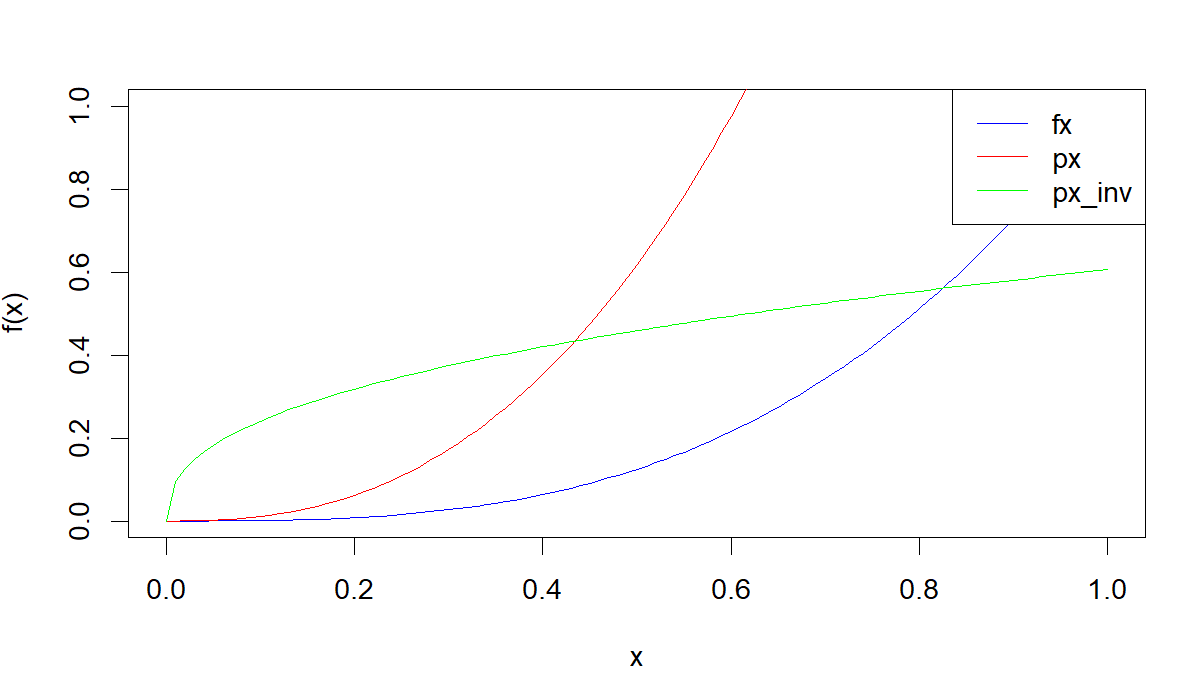
\includegraphics[width=5.60417in,height=\textheight]{qtn1.png}
\caption{Plots of target, proposal and the proposal inverse
distributions}
\end{figure}

\begin{Shaded}
\begin{Highlighting}[]
\CommentTok{\#plot fx }
\NormalTok{x }\OtherTok{\textless{}{-}} \FunctionTok{seq}\NormalTok{(}\DecValTok{0}\NormalTok{, }\DecValTok{1}\NormalTok{, }\FloatTok{0.01}\NormalTok{)}
\NormalTok{y }\OtherTok{\textless{}{-}} \FunctionTok{fx}\NormalTok{(x, }\AttributeTok{n =} \DecValTok{3}\NormalTok{)}
\FunctionTok{plot}\NormalTok{(x, y, }\AttributeTok{type =} \StringTok{"l"}\NormalTok{, }\AttributeTok{col =} \StringTok{"blue"}\NormalTok{, }\AttributeTok{xlab =} \StringTok{"x"}\NormalTok{, }\AttributeTok{ylab =} \StringTok{"f(x)"}\NormalTok{)}

\CommentTok{\# plot the proposal distribution}
\NormalTok{x }\OtherTok{\textless{}{-}} \FunctionTok{seq}\NormalTok{(}\DecValTok{0}\NormalTok{, }\DecValTok{1}\NormalTok{, }\FloatTok{0.01}\NormalTok{)}
\NormalTok{y }\OtherTok{\textless{}{-}} \FunctionTok{px}\NormalTok{(x, k)}
\FunctionTok{lines}\NormalTok{(x, y, }\AttributeTok{col =} \StringTok{"red"}\NormalTok{)}

\CommentTok{\# plot the inverse of the proposal distribution}
\NormalTok{x }\OtherTok{\textless{}{-}} \FunctionTok{seq}\NormalTok{(}\DecValTok{0}\NormalTok{, }\DecValTok{1}\NormalTok{, }\FloatTok{0.01}\NormalTok{)}
\NormalTok{y }\OtherTok{\textless{}{-}} \FunctionTok{px\_inv}\NormalTok{(x, k)}
\FunctionTok{lines}\NormalTok{(x, y, }\AttributeTok{col =} \StringTok{"green"}\NormalTok{)}

\FunctionTok{legend}\NormalTok{(}\StringTok{"topright"}\NormalTok{, }\AttributeTok{legend =} \FunctionTok{c}\NormalTok{(}\StringTok{"fx"}\NormalTok{, }\StringTok{"px"}\NormalTok{, }\StringTok{"px\_inv"}\NormalTok{), }\AttributeTok{col =} \FunctionTok{c}\NormalTok{(}\StringTok{"blue"}\NormalTok{, }\StringTok{"red"}\NormalTok{, }\StringTok{"green"}\NormalTok{), }\AttributeTok{lty =} \DecValTok{1}\SpecialCharTok{:}\DecValTok{1}\NormalTok{)}
\end{Highlighting}
\end{Shaded}

Uniform sampling has a high standard error as it covers the most
rejection area of the target distribution (it is wasteful). Accept
reject sampling has the lowest standard error as it samples from the
proposal distribution and accepts only the values that are close to the
target distribution. Importance sampling has a higher standard error
than accept reject sampling as it samples from the proposal distribution
and places more weight on the values of x that are closer to the target
distribution.

\hypertarget{question-2}{%
\section{Question 2}\label{question-2}}

First we define the target distribution and the proposal distribution.
We then use the metropolis algorithm to sample values from the proposal
distribution and accept or reject the values based on the ratio of the
target and proposal distribution.

\begin{figure}
\centering
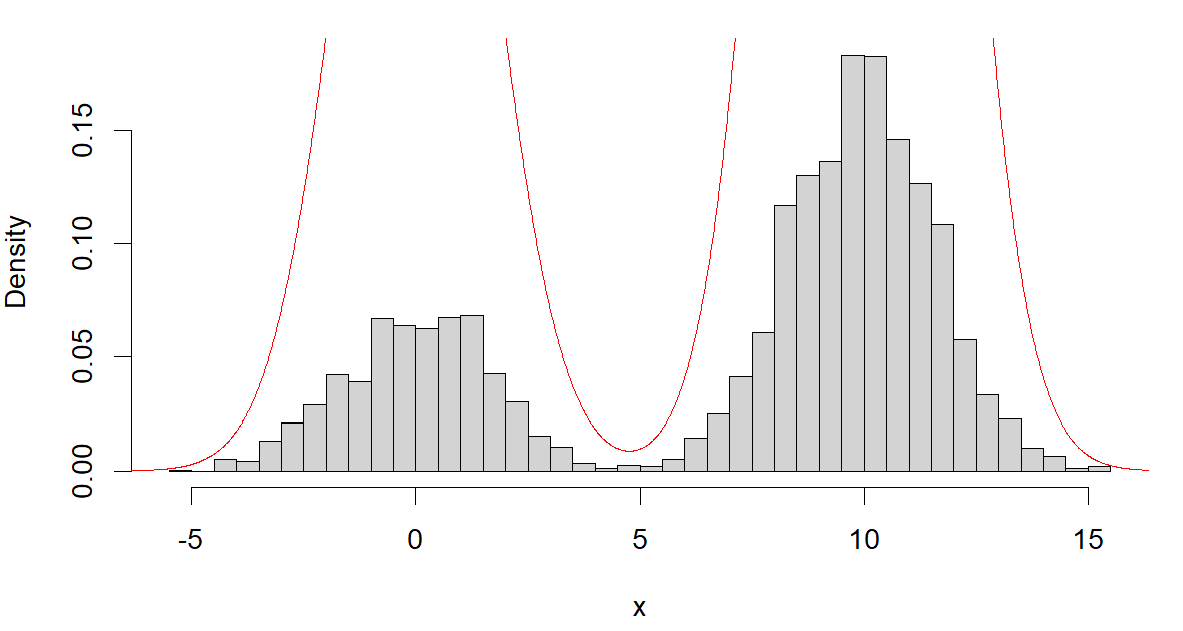
\includegraphics[width=5.58333in,height=\textheight]{qtn2.png}
\caption{Histogram of sampled values, superimposed with min-max
normalized values of p(x)}
\end{figure}

The Markov chain (figure 3)looks like white noise showing that the
samples are independent of each other.

The autocorrelation plot (figure 4) shows that the samples are
independent of each other from the 14th lag onward.

\begin{Shaded}
\begin{Highlighting}[]
\CommentTok{\#metroplis algorithm}

\CommentTok{\#target distribution}
\NormalTok{px }\OtherTok{\textless{}{-}} \ControlFlowTok{function}\NormalTok{(x)\{}
  \FunctionTok{return}\NormalTok{(}\FloatTok{0.3} \SpecialCharTok{*} \FunctionTok{exp}\NormalTok{(}\SpecialCharTok{{-}}\FloatTok{0.2} \SpecialCharTok{*}\NormalTok{ x}\SpecialCharTok{**}\DecValTok{2}\NormalTok{) }\SpecialCharTok{+} \FloatTok{0.7} \SpecialCharTok{*} \FunctionTok{exp}\NormalTok{(}\SpecialCharTok{{-}}\FloatTok{0.2} \SpecialCharTok{*}\NormalTok{ (x }\SpecialCharTok{{-}} \DecValTok{10}\NormalTok{)}\SpecialCharTok{**}\DecValTok{2}\NormalTok{))}
\NormalTok{\}}

\CommentTok{\#proposal distribution}
\NormalTok{sigma }\OtherTok{\textless{}{-}} \DecValTok{10}
\NormalTok{q }\OtherTok{\textless{}{-}} \ControlFlowTok{function}\NormalTok{(x, sigma)\{}
  \FunctionTok{return}\NormalTok{(}\FunctionTok{rnorm}\NormalTok{(}\DecValTok{1}\NormalTok{, x, sigma))}
\NormalTok{\}}
\end{Highlighting}
\end{Shaded}

\begin{Shaded}
\begin{Highlighting}[]
\CommentTok{\#metropolis algorithm}
\FunctionTok{set.seed}\NormalTok{(}\DecValTok{123}\NormalTok{)}
\NormalTok{N }\OtherTok{\textless{}{-}} \DecValTok{5000}
\NormalTok{x }\OtherTok{\textless{}{-}} \FunctionTok{rep}\NormalTok{(}\DecValTok{0}\NormalTok{, N)}
\NormalTok{x[}\DecValTok{1}\NormalTok{] }\OtherTok{\textless{}{-}} \DecValTok{0}
\ControlFlowTok{for}\NormalTok{ (i }\ControlFlowTok{in} \DecValTok{2}\SpecialCharTok{:}\NormalTok{N)\{}
\NormalTok{  x\_star }\OtherTok{\textless{}{-}} \FunctionTok{q}\NormalTok{(x[i}\DecValTok{{-}1}\NormalTok{], sigma)}
\NormalTok{  alpha }\OtherTok{\textless{}{-}} \FunctionTok{min}\NormalTok{(}\DecValTok{1}\NormalTok{, }\FunctionTok{px}\NormalTok{(x\_star)}\SpecialCharTok{/}\FunctionTok{px}\NormalTok{(x[i}\DecValTok{{-}1}\NormalTok{]))}
\NormalTok{  u }\OtherTok{\textless{}{-}} \FunctionTok{runif}\NormalTok{(}\DecValTok{1}\NormalTok{, }\DecValTok{0}\NormalTok{, }\DecValTok{1}\NormalTok{)}
  \ControlFlowTok{if}\NormalTok{ (u }\SpecialCharTok{\textless{}}\NormalTok{ alpha)\{}
\NormalTok{    x[i] }\OtherTok{\textless{}{-}}\NormalTok{ x\_star}
\NormalTok{  \} }\ControlFlowTok{else}\NormalTok{ \{}
\NormalTok{    x[i] }\OtherTok{\textless{}{-}}\NormalTok{ x[i}\DecValTok{{-}1}\NormalTok{]}
\NormalTok{  \}}
\NormalTok{\}}
\end{Highlighting}
\end{Shaded}

\begin{Shaded}
\begin{Highlighting}[]
\CommentTok{\#plot the histogram of the samples}
\FunctionTok{hist}\NormalTok{(x, }\AttributeTok{freq =}\NormalTok{ F, }\AttributeTok{breaks =} \DecValTok{50}\NormalTok{, }\AttributeTok{xlab =} \StringTok{"x"}\NormalTok{, }\AttributeTok{ylab =} \StringTok{"Density"}\NormalTok{)}


\CommentTok{\#superimpose the true distribution}
\NormalTok{x\_tru }\OtherTok{\textless{}{-}} \FunctionTok{seq}\NormalTok{(}\SpecialCharTok{{-}}\DecValTok{10}\NormalTok{, }\DecValTok{20}\NormalTok{, }\FloatTok{0.01}\NormalTok{)}
\NormalTok{y\_tru }\OtherTok{\textless{}{-}} \FunctionTok{px}\NormalTok{(x\_tru)}

\CommentTok{\#min max normalization for the values to be between 0 and 1}
\NormalTok{y\_tru }\OtherTok{\textless{}{-}}\NormalTok{ (y\_tru }\SpecialCharTok{{-}} \FunctionTok{min}\NormalTok{(y\_tru))}\SpecialCharTok{/}\NormalTok{(}\FunctionTok{max}\NormalTok{(y\_tru) }\SpecialCharTok{{-}} \FunctionTok{min}\NormalTok{(y\_tru))}

\FunctionTok{lines}\NormalTok{(x\_tru, y\_tru, }\AttributeTok{col =} \StringTok{"red"}\NormalTok{)}
\end{Highlighting}
\end{Shaded}

\begin{figure}
\centering
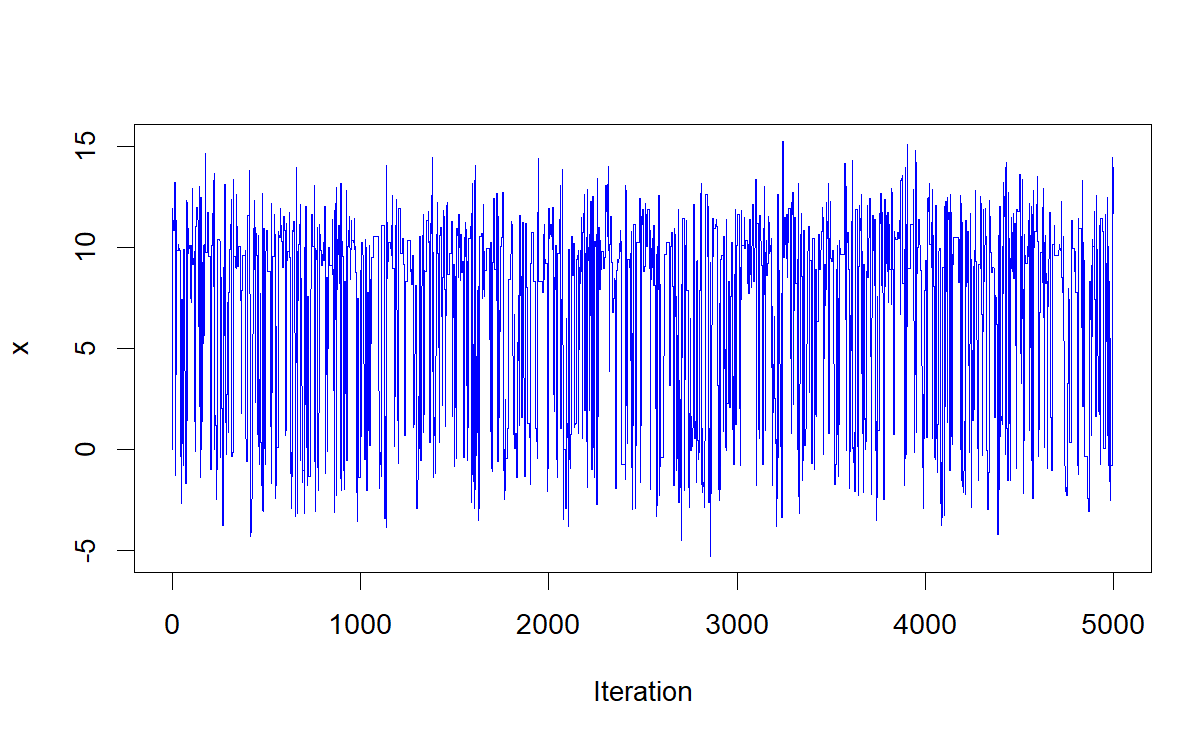
\includegraphics[width=5.40625in,height=\textheight]{markov_chain.png}
\caption{Markov chain}
\end{figure}

\begin{Shaded}
\begin{Highlighting}[]
\CommentTok{\#plot the markov chain}
\FunctionTok{plot}\NormalTok{(x, }\AttributeTok{type =} \StringTok{"l"}\NormalTok{, }\AttributeTok{col =} \StringTok{"blue"}\NormalTok{, }\AttributeTok{xlab =} \StringTok{"Iteration"}\NormalTok{, }\AttributeTok{ylab =} \StringTok{"x"}\NormalTok{)}
\end{Highlighting}
\end{Shaded}

\begin{figure}
\centering
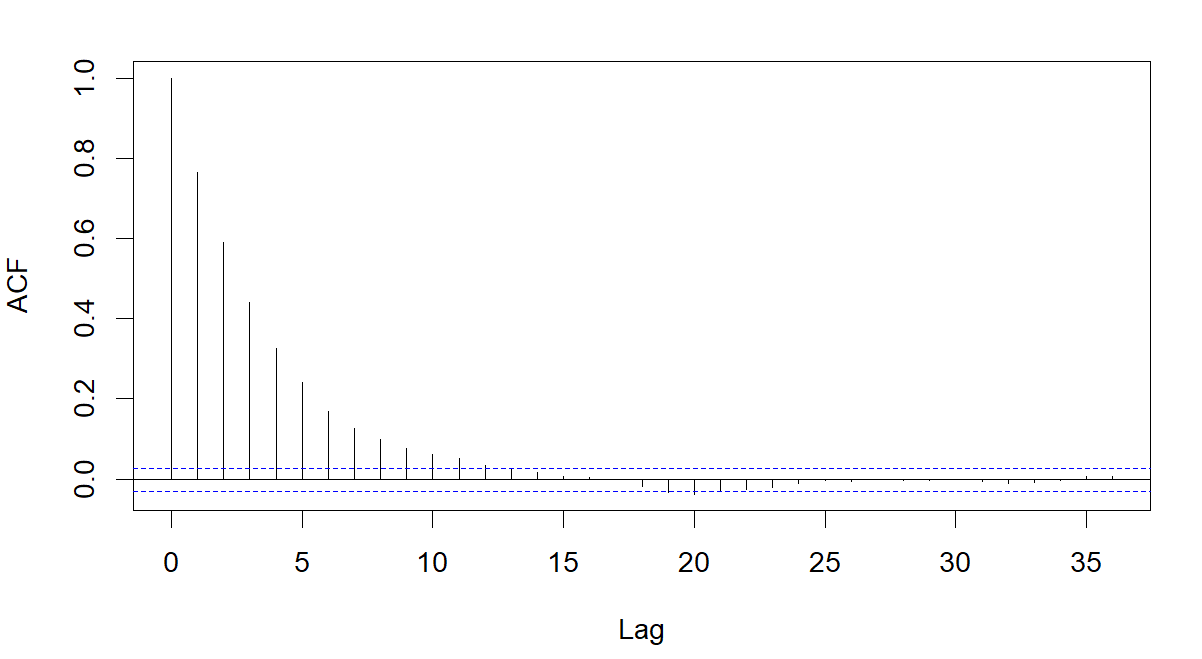
\includegraphics[width=5.59375in,height=\textheight]{acf.png}
\caption{Autocorrelation plot}
\end{figure}

\begin{Shaded}
\begin{Highlighting}[]
\CommentTok{\#plot the autocorrelation}
\FunctionTok{acf}\NormalTok{(x)}
\end{Highlighting}
\end{Shaded}


\end{document}
